\documentclass[../AnalysisNoteJBuxton.tex]{subfiles}
\begin{document}

\section{Correlation Functions}
\label{CorrelationFunctions}

%General remarks about formaton of correlation functions and what information they provide.

This analysis studies the momentum correlations of both $\Lambda$-K and $\Xi$-K pairs using the two-particle correlation function, defined as $C(k^{*}) = A(k^{*})/B(k^{*})$, where $A(k^{*})$ is the signal distribution, $B(k^{*})$ is the reference (or background) distribution, and $k^{*}$ is the momentum of one of the particles in the pair rest frame.
In practice, $A(k^{*})$ is constructed by binning in $k^{*}$ pairs from the same event.
Ideally, $B(k^{*})$ is similar to $A(k^{*})$ in all respects excluding the presence of femtoscopic correlations \cite{Lisa:2005dd}; as such, $B(k^{*})$ is used to divide out the phase-space effects, leaving only the femtoscopic effects in the correlation function. 

In practice, $B(k^{*})$ is obtained by forming mixed-event pairs, i.e. particles from a given event are paired with particles from N$_{mix}$(= 5) other events, and these pairs are then binned in $k^{*}$.
In forming the background distribution, it is important to mix only similar events; mixing events with different phase-spaces can lead to artificial signals in the correlaton function.
Therefore, in this analysis, we mix events with primary vertices within 2 cm and centralities within 5\% of each other.
Also note, a vertex correction is also applied to each event, which essentially recenters the the primary vertices to z = 0.

This analysis presents correlation functions for three centrality bins (0-10\%, 10-30\%, and 30-50\%), and is currently pair transverse momentum ($k_{T} = 0.5|\mathbf{p}_{T,1}+\mathbf{p}_{T,2}|$) integrated (i.e. not binned in $k_{T}$).  
The correlation functions are constructed separately for the two magnetic field configurations, and are combined using a weighted average:

\begin{equation}
  C_{combined}(k^{*}) = \frac{\sum\limits_{i}w_{i}C_{i}(k^{*})}{\sum\limits_{i}w_{i}} 
\label{eqn:CombineCfs}
\end{equation}

where the sum runs over the correlation functions to be combined, and the weight, $w_{i}$, is the number of numerator pairs in $C_{i}(k^{*})$.
Here, the sum is over the two field configurations.

Figures \ref{fig:cLamK0Cfs}, \ref{fig:LamKchPwConjCfs}, and \ref{fig:LamKchMwConjCfs} show the correlation functions for all centalities studied for $\Lambda$K$^{0}_{S}$($\bar{\Lambda}$K$^{0}_{S}$), $\Lambda$K$^{+}$($\bar{\Lambda}$K$^{-}$), and $\Lambda$K$^{-}$($\bar{\Lambda}$K$^{+}$), respectively. All were normalized in the range 0.32 $< k^{*} < $ 0.4 GeV/c.

\begin{figure}[h]
  \centering
  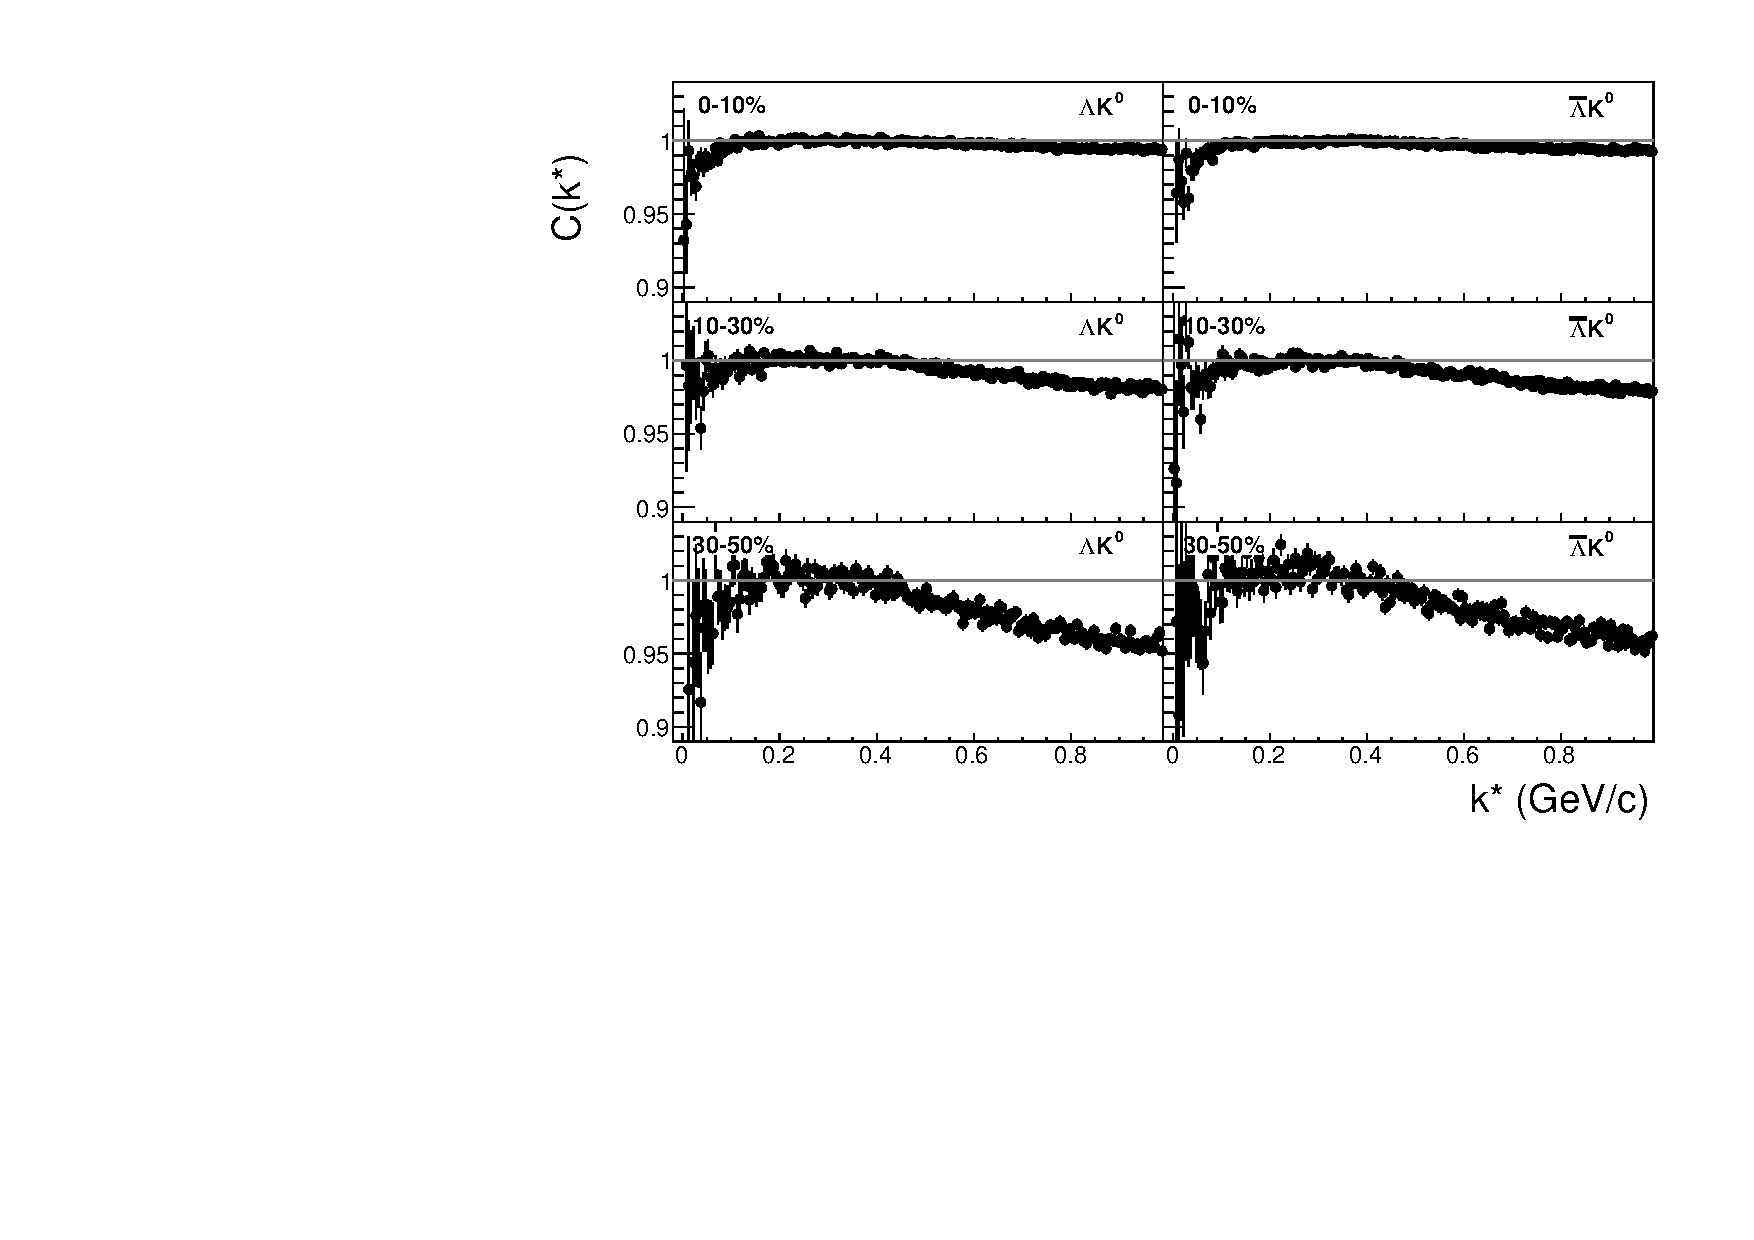
\includegraphics[width=\textwidth]{4_CorrelationFunctions/Figures/canKStarCfsLamK0wConj.pdf}
  \caption[$\Lambda$($\bar{\Lambda}$)K$^{0}_{S}$ Correlation Functions]{$\Lambda$K$^{0}_{S}$ (left) and $\bar{\Lambda}$K$^{0}_{S}$ (right) correlation functions for 0-10\% (top), 10-30\%(middle), and 30-50\%(bottom) centralities.  The lines represent the statistical errors, while the boxes represent the systematic errors.}
  \label{fig:cLamK0Cfs}
\end{figure}

\begin{figure}[h]
  \centering
  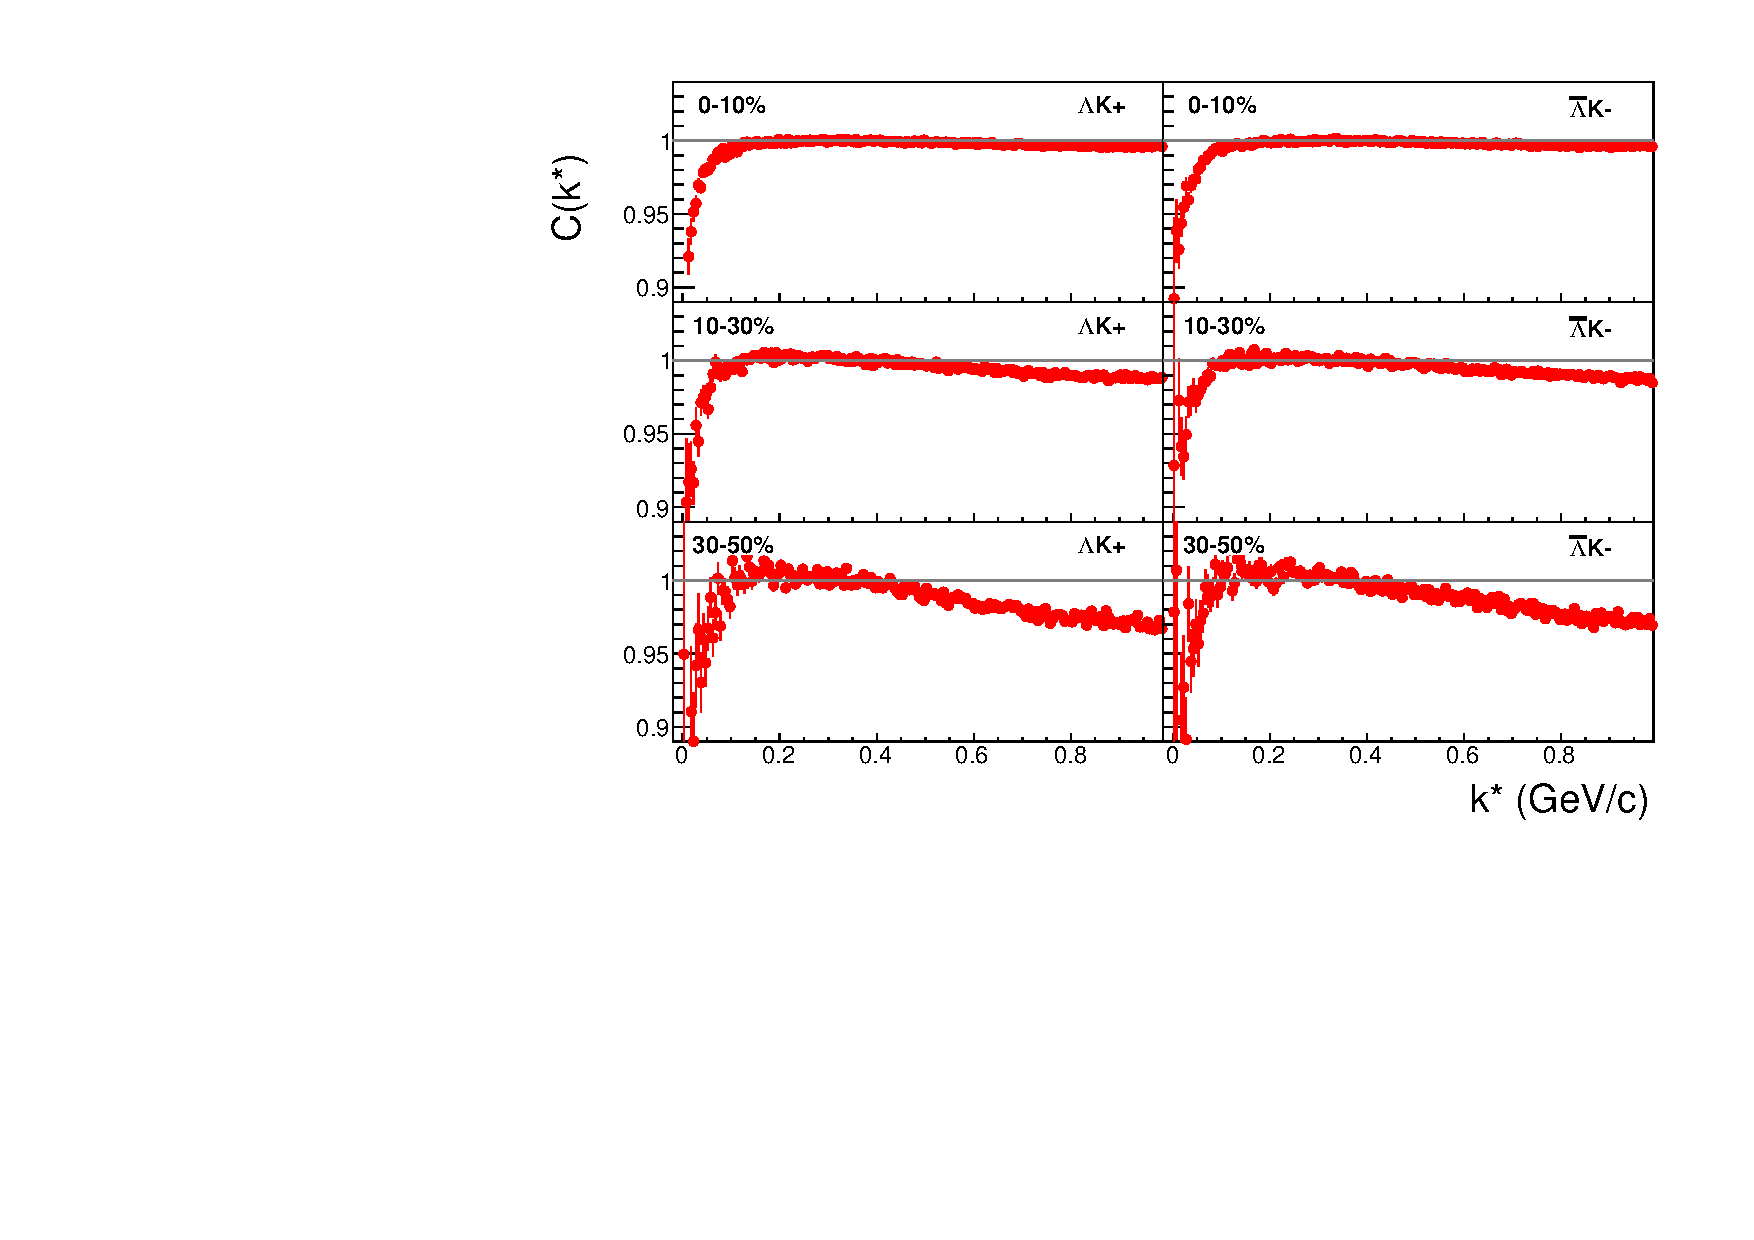
\includegraphics[width=\textwidth]{4_CorrelationFunctions/Figures/canKStarCfsLamKchPwConj.pdf}
  \caption[$\Lambda$K$^{+}$ and $\bar{\Lambda}$K$^{-}$ Correlation Functions]{$\Lambda$K$^{+}$ (left) and $\bar{\Lambda}$K$^{-}$ (right) correlation functions for 0-10\% (top), 10-30\%(middle), and 30-50\%(bottom) centralities.  The lines represent the statistical errors, while the boxes represent the systematic errors.}
  \label{fig:LamKchPwConjCfs}
\end{figure}

\begin{figure}[h]
  \centering
  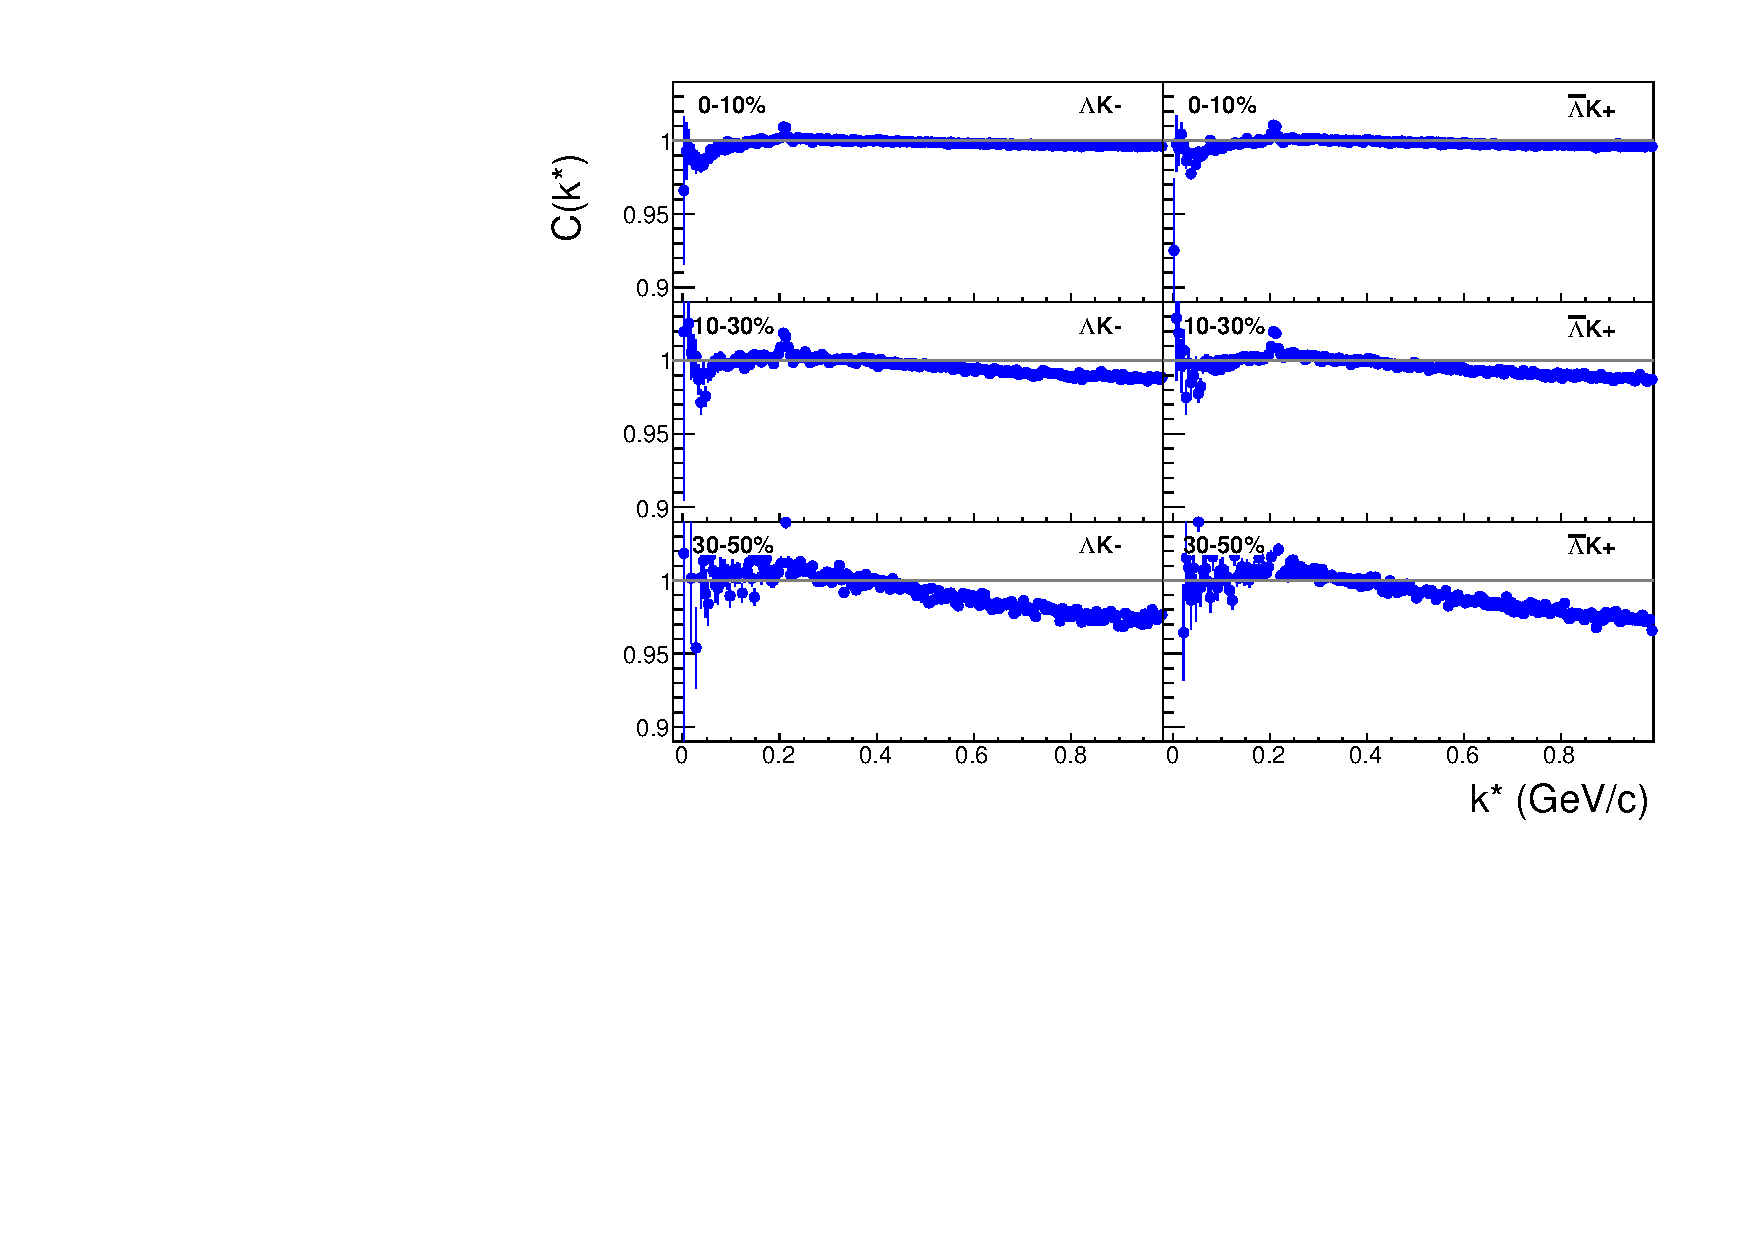
\includegraphics[width=\textwidth]{4_CorrelationFunctions/Figures/canKStarCfsLamKchMwConj.pdf}
  \caption[$\Lambda$K$^{-}$ and $\bar{\Lambda}$K$^{+}$ Correlation Functions]{$\Lambda$K$^{-}$ (left) and $\bar{\Lambda}$K$^{+}$ (right) correlation functions for 0-10\% (top), 10-30\%(middle), and 30-50\%(bottom) centralities.  The lines represent the statistical errors, while the boxes represent the systematic errors.  The peak at k* $\approx$ 0.2 GeV/c is due to the $\Omega^{-}$ resonance.}
  \label{fig:LamKchMwConjCfs}
\end{figure}

\begin{figure}[h]
  \centering
  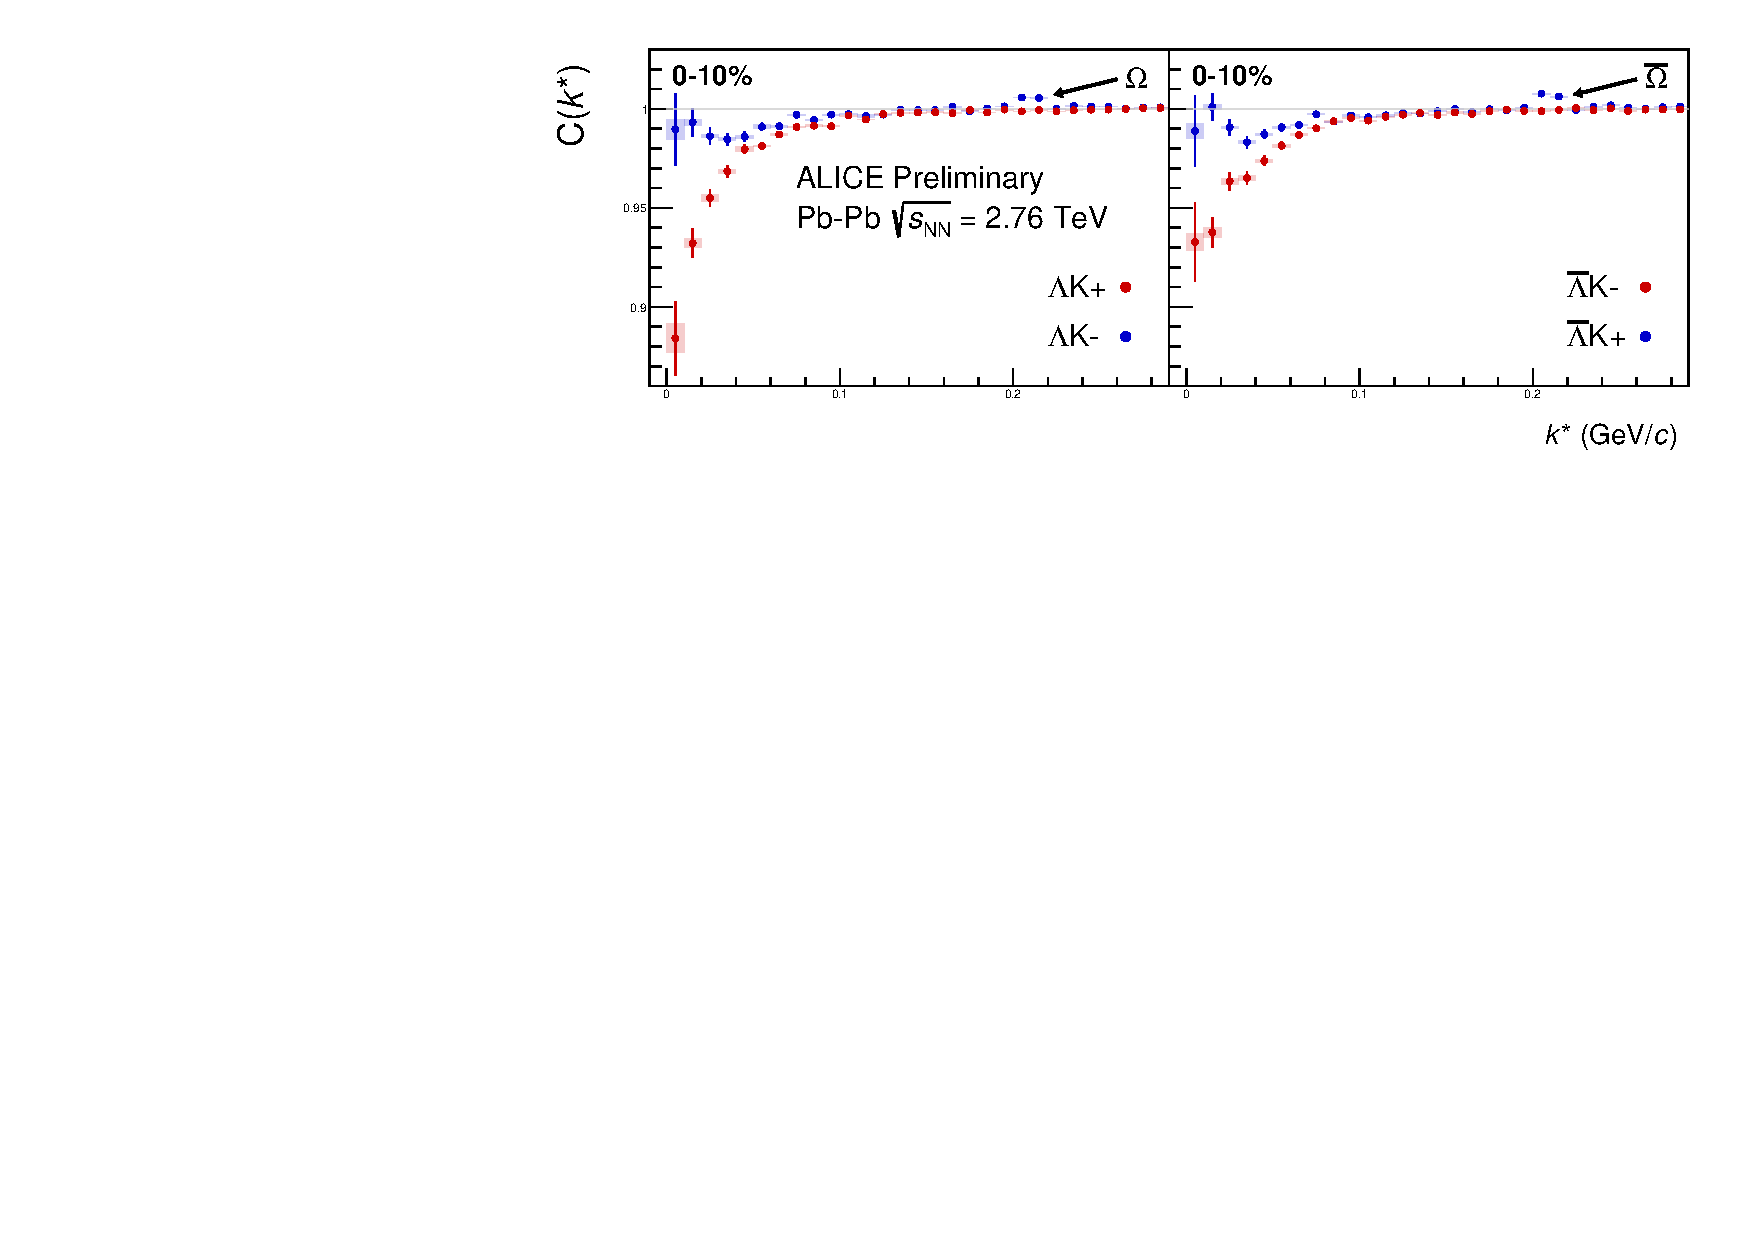
\includegraphics[width=\textwidth]{4_CorrelationFunctions/Figures/canLamKchPvsLamKchM0010.pdf}
  \caption[Correlation Functions: $\Lambda$K$^{+}$ vs $\Lambda$K$^{-}$ for 0-10\% Centrality]{Correlation Functions: $\Lambda$K$^{+}$ vs $\Lambda$K$^{-}$ ($\bar{\Lambda}$K$^{+}$ vs $\bar{\Lambda}$K$^{-}$) for 0-10\% centrality.  The peak in $\Lambda$K$^{-}$($\bar{\Lambda}$K$^{+}$) at k* $\approx$ 0.2 GeV/c is due to the $\Omega^{-}$ resonance.  The lines represent the statistical errors. (NOTE: This figure is slightly dated, and a new one will be generated which includes both statistical and systematic uncertainties)}
  \label{fig:cLamcKchCfs0010}
\end{figure}

\clearpage

\end{document}